\documentclass[12pt]{article}
\usepackage[top=1in,bottom=1in,left=0.75in,right=0.75in,centering]{geometry}
\usepackage{fancyhdr}
\usepackage{epsfig}
\usepackage[pdfborder={0 0 0}]{hyperref}
\usepackage{palatino}
\usepackage{wrapfig}
\usepackage{lastpage}
\usepackage{color}
\usepackage{ifthen}
\usepackage[table]{xcolor}
\usepackage{graphicx,type1cm,eso-pic,color}
\usepackage{hyperref}
\usepackage{amsmath}
\usepackage{wasysym}
\usepackage{amsfonts}
\usepackage{tikz}
\usetikzlibrary{automata, positioning}

\def\course{CS 3120: Discrete Math and Theory II}
\def\homework{Regular Languages}
\def\semester{Fall 2024}

\newboolean{solution}
\setboolean{solution}{false}

% add watermark if it's a solution exam
% see http://jeanmartina.blogspot.com/2008/07/latex-goodie-how-to-watermark-things-in.html
\makeatletter
\AddToShipoutPicture{%
\setlength{\@tempdimb}{.5\paperwidth}%
\setlength{\@tempdimc}{.5\paperheight}%
\setlength{\unitlength}{1pt}%
\put(\strip@pt\@tempdimb,\strip@pt\@tempdimc){%
\ifthenelse{\boolean{solution}}{
\makebox(0,0){\rotatebox{45}{\textcolor[gray]{0.95}%
{\fontsize{5cm}{3cm}\selectfont{\textsf{Solution}}}}}%
}{}
}}
\makeatother

\pagestyle{fancy}

\fancyhf{}
\lhead{\course}
\chead{Page \thepage\ of \pageref{LastPage}}
\rhead{\semester}
%\cfoot{\Large (the bubble footer is automatically inserted into this space)}

\setlength{\headheight}{14.5pt}

\newenvironment{itemlist}{
\begin{itemize}
\setlength{\itemsep}{0pt}
\setlength{\parskip}{0pt}}
{\end{itemize}}

\newenvironment{numlist}{
\begin{enumerate}
\setlength{\itemsep}{0pt}
\setlength{\parskip}{0pt}}
{\end{enumerate}}

\newcounter{pagenum}
\setcounter{pagenum}{1}
\newcommand{\pageheader}[1]{
\clearpage\vspace*{-0.4in}\noindent{\large\bf{Page \arabic{pagenum}: {#1}}}
\addtocounter{pagenum}{1}
\cfoot{}
}

\newcounter{quesnum}
\setcounter{quesnum}{1}
\newcommand{\question}[2][??]{
\begin{list}{\labelitemi}{\leftmargin=2em}
\item [\arabic{quesnum}.] {} {#2}
\end{list}
\addtocounter{quesnum}{1}
}


\definecolor{red}{rgb}{1.0,0.0,0.0}
\newcommand{\answer}[2][??]{
\ifthenelse{\boolean{solution}}{
\color{red} #2 \color{black}}
{\vspace*{#1}}
}

\definecolor{blue}{rgb}{0.0,0.0,1.0}

\begin{document}

\section*{\homework}

\question[3]{
Draw out \emph{DFA}s (not \emph{NFA}s) for each of the following languages. For some of these, a small hint is provided. Your goal is to construct a \emph{DFA} with as few states as possible (just like how we prefer to write succinct code when possible). For all of these, let $\Sigma = \{a,b\}$
}

\begin{itemize}
	\item $\{w \ | \ w \text{ does not contain the substring } abba \}$ (\emph{*Hint: Draw out the DFA for a simpler language that DOES contain abba and then try to change that machine slightly.})

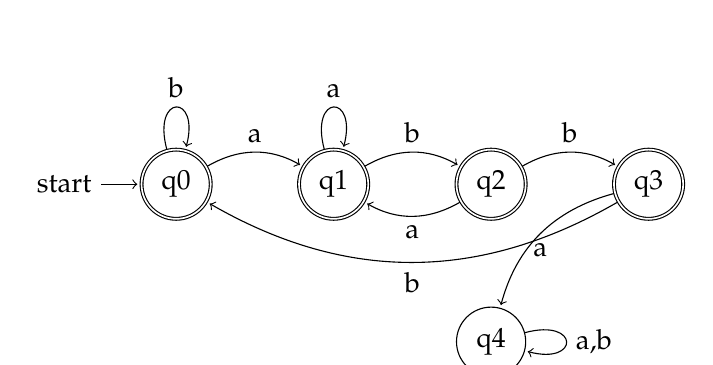
\begin{tikzpicture}[shorten >=1pt, node distance=2cm, on grid, auto]
  % Nodes
  \node[state, initial, accepting] (q0) {q0};
  \node[state, accepting] (q1) [right=of q0] {q1};
  \node[state, accepting] (q2) [right=of q1] {q2};
  \node[state, accepting] (q3) [right=of q2] {q3};
  \node[state] (q4) [below=2cm of q2] {q4};
  % Edges
  \path[->]
    (q0) edge [bend left] node {a} (q1)
         edge [loop above] node {b} ()
    (q1) edge [loop above] node {a} ()
         edge [bend left] node {b} (q2)
    (q2) edge [bend left] node {a} (q1)
         edge [bend left] node {b} (q3)
    (q3) edge [bend right] node [below] {a} (q4)
         edge [bend left] node {b} (q0)
    (q4) edge [loop right] node {a,b} ();
\end{tikzpicture}

	\item $\{w \ | \ w \text{ contains BOTH the substrings ab and ba}\}$

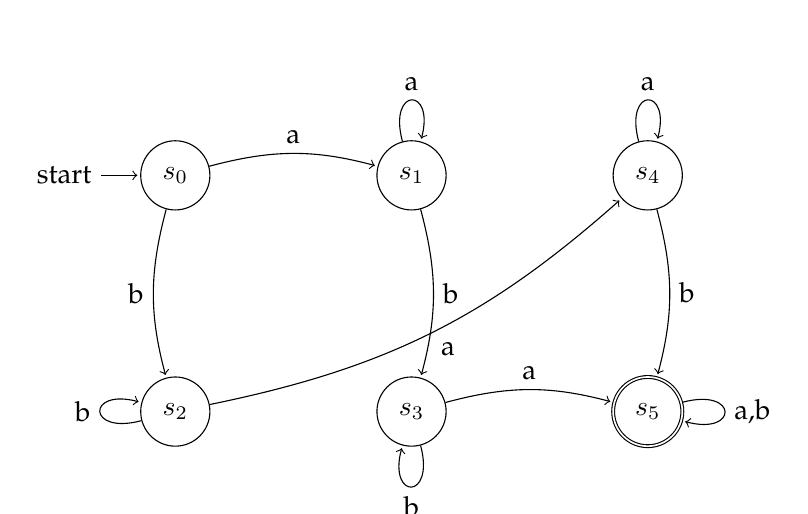
\begin{tikzpicture}[shorten >=1pt, node distance=3cm, on grid, auto] 
   \node[state, initial] (s_0)   {$s_0$}; 
   \node[state] (s_1) [right=of s_0] {$s_1$}; 
   \node[state] (s_2) [below=of s_0] {$s_2$}; 
   \node[state] (s_3) [right=of s_2] {$s_3$}; 
   \node[state] (s_4) [right=of s_1] {$s_4$}; 
   \node[state, accepting] (s_5) [below=of s_4] {$s_5$}; 

    \path[->] 
    (s_0) edge [bend left=15] node {a} (s_1)
          edge [bend right=15] node [swap] {b} (s_2)
    (s_1) edge [loop above] node {a} (s_1)
          edge [bend left=15] node {b} (s_3)
    (s_2) edge [loop left] node {b} (s_2)
          edge [bend right=15] node [swap] {a} (s_4)
    (s_3) edge [loop below] node {b} (s_3)
          edge [bend left=15] node {a} (s_5)
    (s_4) edge [loop above] node {a} (s_4)
          edge [bend left=15] node {b} (s_5)
    (s_5) edge [loop right] node {a,b} (s_5);
\end{tikzpicture}

	\item $\{w \ | \ w \in a^*b^*a^* \}$

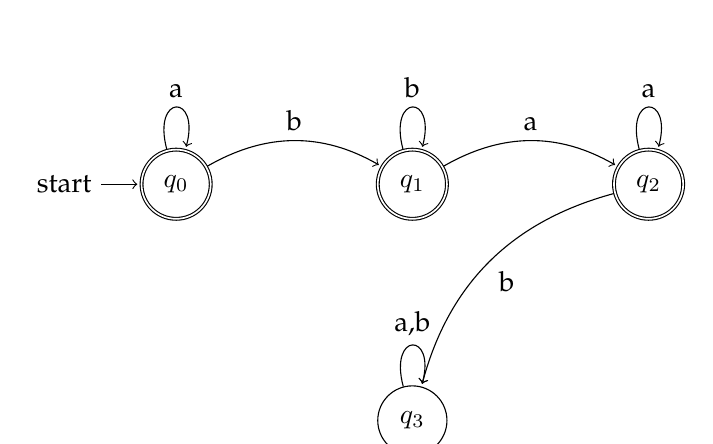
\begin{tikzpicture}[shorten >=1pt, node distance=3cm, on grid, auto]

  % States
  \node[state, initial, accepting] (q0) {$q_0$};  % Initial and accepting state
  \node[state, accepting] (q1) [right of=q0] {$q_1$}; % State for reading b's
  \node[state, accepting] (q2) [right of=q1] {$q_2$}; % State for reading a's after b's
  \node[state] (q3) [below of=q1] {$q_3$};  % Fixed label for q3

  % Transitions
  \path[->]
    (q0) edge [loop above] node {a} ()          % q0 loops on 'a'
         edge [bend left] node {b} (q1)         % q0 goes to q1 on 'b'
    (q1) edge [loop above] node {b} ()          % q1 loops on 'b'
         edge [bend left] node {a} (q2)         % q1 goes to q2 on 'a'
    (q2) edge [loop above] node {a} ()          % q2 loops on 'a'
         edge [bend right] node {b} (q3)      % q2 goes to trap on 'b'
    (q3) edge [loop above] node {a,b} ();     % trap loops on both 'a' and 'b'

\end{tikzpicture}

	\item $\{w \ | \ w \neq ab \wedge w \neq bb \}$

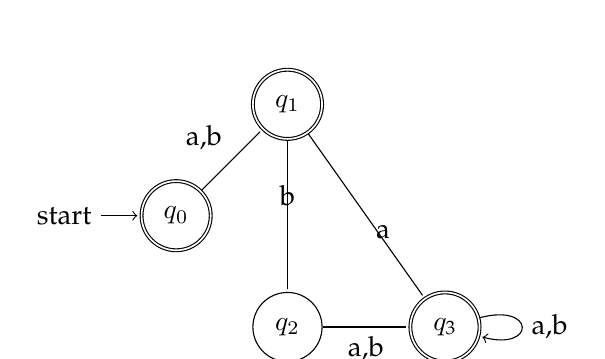
\begin{tikzpicture}[shorten >=1pt,node distance=2cm,on grid,auto]
    \node[state,initial,accepting] (q0) {$q_0$};
    \node[state,accepting] (q1) [above right of=q0] {$q_1$};
    \node[state] (q2) [below right of=q0] {$q_2$};
    \node[state,accepting] (q3) [right of=q2] {$q_{\text{3}}$};

    \path
    (q0) edge node[above left] {a,b} (q1)
    (q1) edge[below right] node {a} (q3)
         edge node[above] {b} (q2)
    (q2) edge node[below] {a,b} (q3)
    (q3) edge[loop right] node {a,b} (q3);
\end{tikzpicture}

	\item $\{w \ | \ w \in a^iw' \ | \ i \in \mathbb{N}, w' \in \{a,b\}^*, \text{w' contains at least i a's} $ (\emph{*Hint: This one LOOKS not regular but it actually is. Can you figure out why?})

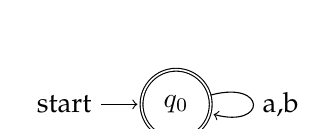
\begin{tikzpicture}[shorten >=1pt,node distance=2cm,on grid,auto]

\node[state,initial,accepting] (q0) {$q_0$};

\path
    (q0) edge[loop right] node {a,b} (q0);
\end{tikzpicture}

\end{itemize}

\vspace{12pt}

\question[3]{
Prove that regular languages are closed under \emph{intersection}. Do this by starting with \emph{DFA}s for two regular languages $A$ and $B$, and describe how to construct a new \emph{DFA} for $A \cap B$\
\\

We start with two regular languages A and B, whose DFA's can be represented as $M_A = (Q_A, \Sigma, \delta_A, q_{A0}, F_A)$ and $M_B = (Q_B, \Sigma, \delta_B, q_{B0}, F_B)$. To construct a new DFA for $A \cap B$, say $M_C = (Q_A $ x $ Q_B, \Sigma, (\delta_A(q_A,a),\delta_A(q_A,a)) ,F_A $ x $ F_B)$, such that we would need to take the cross product and get all pairs of states and a transition function that simulates transitions for both DFAs $M_A $ and $ M_B$.\\
\\
Let w be any string in $\Sigma*$, we need to show that w $\in$ a language, $C$, accepted by $M_C$. If w exists in the set $A \cap B$, then it must reach accepting states in both A and B, such that $q_A \in F_A$ and $q_B \in F_B$ where $F_C$ will reach a state $(q_A, q_B)$. The string $w$ will be apart of the language $C$ by construction of the DFA for $C$ as it will only accept strings to be part of the language if it is in languages $A$ and $B$.
}

%\delta((q_{A0}, q_{B0}), a) = 

\vspace{12pt}

\question[3]{
Prove that regular languages are closed under \emph{complement}. Do this by starting with a \emph{DFA} for a regular language $A$, and describe how to construct a new \emph{DFA} for $\bar{A}$.
\\

Let $M = (Q_A, \Sigma, \delta, q_0, F_A)$ be a DFA for the regular language $A$, where $Q_A$ is the set of states, $\Sigma$ is the alphabet, $\delta$ is the transition function, $q_0$ is the start state, and $F_A$ is the set of accepting states.\\
\\
To construct a DFA for the complement of $A$, denoted $\bar{A}$, we define a new DFA $M' = (Q_A, \Sigma, \delta, q_0, Q_A \setminus F_A)$. In this new DFA, the set of accepting states is $Q_A \setminus F_A$, meaning all states in $Q_A$ that were not accepting in $A$ are now accepting in $M'$.\\
\\
For any string $w$, if $w$ is in the language $A$, it is accepted by $M$, meaning the state reached after processing $w$ is in $F_A$. However, in $M'$, this same string $w$ will be rejected, as $w$ leads to a state that is not in the accepting set of $M'$. Conversely, if $w$ is not in $A$, it will be accepted by $M'$. This construction proves that the complement of a regular language is also regular.
}

\vspace{12pt}

\question[3]{
For any string $w = w_1w_2,...,w_n$, let $w^R$ be the reverse of string $w$ (i.e., $w^R=w_n,...,w_2,w_1$). Prove that if a language $A$ is regular, then the language $A^R = \{w^R \ | \ w \in A\}$ is also regular.


}

Since \( A \) is a regular language, there exists a DFA \( M = (Q, \Sigma, \delta, q_0, F) \) that recognizes \( A \), where:

\begin{itemize}
    \item \( Q \) is the set of states,
    \item \( \Sigma \) is the input alphabet,
    \item \( \delta: Q \times \Sigma \to Q \) is the transition function,
    \item \( q_0 \in Q \) is the initial state, and
    \item \( F \subseteq Q \) is the set of accepting states.
\end{itemize}

Now, we need to show that there exists a finite automaton that recognizes the language \( A^R = \{ w^R \mid w \in A \} \).

\subsection*{Step 1: Reverse the DFA}
We will construct a new automaton \( M^R \) that recognizes \( A^R \). We will do this by reversing the transitions of \( M \). This means the accept states will become the initial states and the initial states become the accepting states. Specifically:

\begin{enumerate}
    \item Reverse all transitions in \( M \), for every transition \( \delta(q, a) = q' \), add a reverse transition \( \delta^R(q', a) = q \) in the new automaton \( M^R \).
    \item Make each accepting state in \( F \) an initial state in \( M^R \).
    \item The initial state \( q_0 \) in \( M \) will become the only accepting state in \( M^R \).
\end{enumerate}

\subsection*{Step 2: NFA}
Since the reversed transitions of \( M\) may lead to multiple possible states, \( M^R \) is a NFA.

The NFA, \( M^R = (Q, \Sigma, \delta^R, F, \{q_0\}) \) has:
\begin{itemize}
    \item The same set of states \( Q \)
    \item The same input alphabet \( \Sigma \)
    \item The reversed transition function \( \delta^R \)
    \item The set of initial states \( F \), the accepting states in \( M \)
    \item The set of accepting states \( \{q_0\} \), the start state of \( M \)
\end{itemize}

\subsection*{Step 3: \( A^R \)}
We know that NFAs and DFAs recognize the same class of languages, regular languages. Therefore, the language recognized by \( M^R \), which is \( A^R \), is regular because we can convert any NFA to an equivalent DFA.

\subsection*{Conclusion}
Since we have constructed an NFA that recognizes \( A^R \), and regular languages are closed under reversal, we conclude that if \( A \) is regular, then \( A^R \) is also regular.

\vspace{12pt}

\question[3]{
Use the pumping lemma to show that the following languages are not regular OR argue that they are regular. 
}

\begin{itemize}
	\item $A= \{ 0^*0^n1^n1^* \ | \ n \geq 0\}$\\
\\
Assume that language $A$ is regular.\\
\\
By the pumping lemma, there exists a pumping length $p$ such that any string $s$ in the language $A$ of length at least $p$ can be divided into three parts $s = xyz$ satisfying the following conditions:
\begin{itemize}
    \item for each $i \geq 0, xy^iz \in A$,
    \item $|y| > 0$,
    \item $|xy| \leq p$.
\end{itemize}

In this case, let us select the string $s' = 0^p1^p$, which follows the form required by language $A$ and is structured such that we have $p$ zeros followed by $p$ ones.\\

According to the pumping lemma, $s'$ can be divided into $s' = xyz$, where we can "pump" $y$ any number of times, $|y| > 0$, and $|xy| \leq p$. Based on this, there are three potential cases to consider:

\begin{itemize}
    \item $y$ contains only 0s: If $y$ consists only of 0s from the first block of $0^p$, pumping $y$ will increase or decrease the number of 0s in this block. The resulting string, then, would look like $0^{p+k}1^p$, where $k$ is the number of 0s added or removed, which breaks the balance between the number of 0s and 1s, thereby contradicting the structure of the language.
    
    \item $y$ contains some 0s and some 1s: If $y$ contains both 0s and 1s, pumping $y$ will mix the 0s and 1s, disrupting the boundary between the block of 0s and the block of 1s. The resulting string would look like $0^{p-k}1^{p+k}$, which is not of the form $0^n1^n$, thereby contradicting the structure of the language.
    
    \item $y$ contains only 1s: If $y$ consists only of 1s from the second block of $1^p$, pumping $y$ will increase or decrease the number of 1s in this block. The resulting string, then, would look like $0^p1^{p+k}$, where $k$ is the number of 1s added or removed, which breaks the balance between the number of 0s and 1s, thereby contradicting the structure of the language.
\end{itemize}

In all three cases, pumping $y$ results in a string that violates the structure of the language $A$. Whether $y$ contains only 0s, both 0s and 1s, or only 1s, the resulting string after pumping does not preserve the required balance between the blocks of 0s and 1s. As such, we have found a valid string $s'$ that cannot be pumped without breaking the conditions of the language. Thus, this contradicts the assumption that $A$ is regular, and we can conclude that language $A$ is not regular.

	\item $B= \{ www \ | \ w \in \{0,1\}^* \}$\\
\\
Assume that language $B$ is regular.\\

By the pumping lemma, there exists a pumping length $p$ such that any string $s$ in the language $B$ of length at least $p$ can be divided into three parts $s = xyz$ satisfying the following conditions:
\begin{itemize}
    \item for each $i \geq 0, xy^iz \in B$,
    \item $|y| > 0$,
    \item $|xy| \leq p$.
\end{itemize}

In this case, let us select the string $s' = 0^p10^p10^p$, which consists of three consecutive copies of the substring $0^p$ with $1$ separating each substring instance (and consequently follows the form $www$ required by the language $B$), making it a valid string in $B$.\\

According to the pumping lemma, $s'$ can be divided into $s' = xyz$, where we can "pump" $y$ any number of times, $|y| > 0$, and $|xy| \leq p$. Based on this, there are three potential cases to consider:

\begin{itemize}
    \item $y$ contains only 0s: If $y$ consists only of 0s from the first block of $0^p$, pumping $y$ will increase or decrease the number of 0s in this block. The resulting string, then, would look like $0^{p+k}10^p10^p$, where $k$ is the number of 0s added or removed. This string is no longer of the form $www$, as the first part is no longer the same as the subsequent parts, thereby contradicting the structure of the language.
    
    \item $y$ contains a 1 and some 0s: If $y$ contains a 1 and some 0s, spanning across the boundary between the second block of $0^p$ and the first 1, pumping $y$ will mix 0s and the 1, resulting in a string like $0^{p-k}110^p10^p$. This string disrupts the pattern $www$ because the middle copy of $w$ no longer starts with the same 0s, thereby violating the required repetition of $w$.
    
    \item $y$ contains some 0s and a 1: If $y$ consists of some 0s and the 1 from the second block of $0^p$, pumping $y$ will change the structure of the second occurrence of $w$. The resulting string would look like $0^p1^k0^{p-k}10^p$, which again does not maintain the required repetition of $w$, leading to a contradiction.
\end{itemize}

In all three cases, pumping $y$ results in a string that violates the structure of the language $B$. Whether $y$ contains only 0s, a 1 and some 0s, or some 0s and a 1, the resulting string after pumping does not maintain the repetition required by the language $B$. As such, we have found a valid string $s'$ that cannot be pumped without breaking the conditions of the language. Thus, this contradicts the assumption that $B$ is regular, and we can conclude that language $B$ is not regular.
\end{itemize}

\vspace{12pt}

\question[3]{
Find and describe the error that exists in the following proof. The proof attempts to show that $0^*1^*$ is not regular, when in fact it is:
\\
\\
\emph{
Assume, for sake of contradiction, that $0^*1^*$ is regular. We select an element from this language that is greater than the pumping length $p$. We select $0^p1^p$. In class, when proving that $0^n1^n$ was not regular, we showed that $0^p1^p$ cannot be pumped. Therefore, $0^*1^*$ is not regular.
}
\\
\\
The error in the proof lies in a misunderstanding of the language $0^*1^*$ and a misapplication of the pumping lemma in an attempt to show that $0^*1^*$ is not regular. For context, the pumping lemma for regular languages states that for any regular language $A$, there exists a pumping length $p$ such that any string $s \in A$ where $|s| \geq p$ can be divided into three parts $s = xyz$ satisfying the following conditions:
\begin{itemize}
    \item for each $i \geq 0, xy^iz \in A$,
    \item $|y| > 0$,
    \item $|xy| \leq p$.
\end{itemize}

In this case, the proof incorrectly references this concept to select the string $s' = 0^p1^p$ from the language $0^*1^*$ and assumes that this string cannot be pumped, following the reasoning outlined in class to prove that $0^n1^n$ is not regular. However, $0^*1^*$ is a different language with a simpler structure than $0^n1^n$, allowing any number of $0$s followed by any number of $1$s as opposed to requiring the number of $0$s to exactly match the number of $1$s; accordingly, the string $0^p1^p$ can indeed be pumped within this language.\\
\\
For example, if we divide $s'$ such that $s' = xyz$ and select $y$ to be a section of $s'$ containing only $0$s (e.g., $y = 0^k$ for some $k > 0$), we will always be able to pump $y$ by repeating or omitting occurrences of $0$s (i.e., consider strings $0^{p+k}1^p$ or $0^{p-k}1^p$), and the resulting strings will still belong to $0^*1^*$. Similarly, if we select $y$ to be a section of $s'$ containing only $1$s (e.g., $y = 1^k$ for some $k > 0$), we will always be able to pump $y$ by repeating or omitting occurrences of $1$s (i.e., consider strings $0^p1^{p+k}$ or $0^p1^{p-k}$); through this logic, we see that the selected string $s' = 0^p1^p$ can be pumped and will still fit within the structure of the language. Furthermore, pumping $y$ in any case still produces a valid string in $0^*1^*$, as it merely changes the number of $0$s and/or the number of $1$s while retaining the structure of some number of $0$s followed by some number of $1$s, which is allowed by the language.\\
\\
Conclusively, the root issue in the proof is the incorrect assumption that the language $0^*1^*$ behaves like the language $0^n1^n$, where the number of $0$s must match the number of $1$s. Instead, with $0^*1^*$, there is no such restriction on the relationship between the number of $0$s and the number of $1$s, meaning that the pumping lemma can be applied without generating strings that fall outside the language. Thus, the proof fails in its attempt to employ similar rationale showing that the language $0^n1^n$ is not regular to show that the language $0^*1^*$ is also not regular, when, in fact, it is regular.
}

\vspace{12pt}


\end{document}
